\documentclass{article}

\usepackage[svgnames]{xcolor}
\usepackage{listings}
\usepackage[utf8]{inputenc}
\usepackage[T1]{fontenc}

\lstset{language=R,
    basicstyle=\small\ttfamily,
    stringstyle=\color{DarkGreen},
    otherkeywords={0,1,2,3,4,5,6,7,8,9},
    morekeywords={TRUE,FALSE},
    deletekeywords={data,frame,length,as,character},
    keywordstyle=\color{blue},
    commentstyle=\color{DarkGreen},
}

\usepackage{Sweave}
\begin{document}
\Sconcordance{concordance:mlppacotes.tex:mlppacotes.Rnw:%
1 17 1 1 0 24 1 1 154 156 0 1 2 4 1 1 37 39 0 1 2 4 1 1 34 36 0 1 2 4 1 %
1 2 1 0 1 1 7 0 1 2 2 1 1 2 1 0 1 1 7 0 1 2 2 1 1 2 6 0 1 1 7 0 1 2 1 1}


\title{MLP Pacotes}
\author{Matheus Araujo - 2013066265}
\date{}

\maketitle

O objetivo da atividade dessa semana é avaliar o desempenho de três diferentes métodos de treinamento na solução de um mesmo problema.

O problema escolhido para avaliação foi o de aproximação linear da função seno.

Os métodos avaliados foram:

\begin{itemize}
  \item Método 1 - Backpropagation, implementado na Atividade 6.
  \item Método 2 - Elman, do pacote RSNNS
  \item Método 3 - Neuralnet, do pacote Neuralnet
\end{itemize}

\section{Método 1}

A função \texttt{avaliarMetodo1}, já implementada com o nome de \texttt{rnaSeno} na Atividade 6, é apresentada seguir.

\begin{Schunk}
\begin{Sinput}
> avaliarMetodo1 <- function() {
+ 
+   rm(list=ls())
+ 
+   sech2<-function(u)
+   {
+     return(((2/(exp(u)+exp(-u)))*(2/(exp(u)+exp(-u))))) 
+   }
+ 
+   # dados de entrada
+   x_train<-seq(from=0, to=2*pi, by=0.15)
+   x_train<-x_train + (runif(length(x_train))-0.5)/5
+   i <- sample(length(x_train))
+   x_train <- x_train[i]
+ 
+   y_train <- sin(x_train)
+   y_train<-y_train + (runif(length(y_train))-0.5)/5
+ 
+   x_test <-seq(from=0, to=2*pi, by =0.01)
+   y_test <-sin(x_test)
+ 
+   # pesos de entrada
+   i1<-1
+   i2<-1
+   i3<-1
+   i4<-1
+ 
+   w61<-runif(1)-0.5
+   w65<-runif(1)-0.5
+ 
+   w72<-runif(1)-0.5
+   w75<-runif(1)-0.5
+ 
+   w83<-runif(1)-0.5
+   w85<-runif(1)-0.5
+ 
+   w94<-runif(1)-0.5
+   w96<-runif(1)-0.5
+   w97<-runif(1)-0.5
+   w98<-runif(1)-0.5
+ 
+   tol<-0.01
+   nepocas<-0
+   eepoca<-tol+1
+   eta<-0.01
+   maxepocas<-50000
+ 
+   evec<-matrix(nrow=1,ncol=maxepocas) 
+ 
+   while ((nepocas < maxepocas) && (eepoca>tol)){
+     ei2<-0
+     iseq<-sample(length(x_train))
+     for(i in (1:length(x_train))) {
+     
+       i5<-x_train[iseq[i]]
+       y9<-y_train[iseq[i]]
+       
+       u6<-i1*w61+i5*w65
+       i6<-tanh(u6)
+       
+       u7<-i2*w72+i5*w75
+       i7<-tanh(u7)
+       
+       u8<-i3*w83+i5*w85
+       i8<-tanh(u8)
+       
+       u9<-i4*w94+i6*w96+i7*w97+i8*w98
+       i9<-u9
+       
+       e9<-y9-i9
+       
+       d9<-e9
+       
+       dw94<-eta*d9*i4
+       dw96<-eta*d9*i6
+       dw97<-eta*d9*i7
+       dw98<-eta*d9*i8
+ 
+       d6<-sech2(u6)*(d9*w96)
+       d7<-sech2(u7)*(d9*w97)
+       d8<-sech2(u8)*(d9*w98)
+       
+       dw61<-eta*d6*i1
+       dw65<-eta*d6*i5
+ 
+       dw72<-eta*d7*i2
+       dw75<-eta*d7*i5
+ 
+       dw83<-eta*d8*i3
+       dw85<-eta*d8*i5
+ 
+       w61<-w61+dw61
+       w65<-w65+dw65
+ 
+       w72<-w72+dw72
+       w75<-w75+dw75
+ 
+       w83<-w83+dw83
+       w85<-w85+dw85
+ 
+       w94<-w94+dw94
+       w96<-w96+dw96
+       w97<-w97+dw97
+       w98<-w98+dw98
+ 
+       ei<-e9*e9
+       ei2<-ei2+ei
+     }
+     
+     nepocas<-nepocas+1 
+     evec[nepocas]<-ei2
+     eepoca<-evec[nepocas]
+   }
+ 
+   x_calc<-x_test
+   y_calc<-y_test
+ 
+   for(i in (1:length(x_test))) {
+     i5<-x_test[i]
+ 
+     u6<-i1*w61+i5*w65
+     i6<-tanh(u6)
+ 
+     u7<-i2*w72+i5*w75
+     i7<-tanh(u7)
+ 
+     u8<-i3*w83+i5*w85
+     i8<-tanh(u8)
+ 
+     u9<-i4*w94+i6*w96+i7*w97+i8*w98
+     i9<-u9
+ 
+     y_calc[i]<-i9
+ 
+   }
+ 
+   n_test<-length(x_test)
+   erro<-0
+   for(i in 1:n_test)
+     erro<-erro + (y_test[i]-y_calc[i])^2
+ 
+   erro<-erro/n_test
+   erro  
+ 
+   retlist<-list(erro, nepocas, evec[(1:nepocas)], x_test, y_test, y_calc)
+ 
+   plot(x_test, y_test, type='l', col='black', xlab='x', ylab='y1')
+   par(new=T)
+   plot(x_test, y_calc, type='l', col='blue', xlab='', ylab='')
+   
+   return (erro)
+ 
+ }
\end{Sinput}
\end{Schunk}

\section{Método 2}

A função \texttt{avaliarMetodo2} é apresentada a seguir

\begin{Schunk}
\begin{Sinput}
> avaliarMetodo2 <- function() {
+   rm(list=ls())
+   
+   library("RSNNS")
+ 
+   # dados de entrada
+   x_train<-seq(from=0, to=2*pi, by=0.15)
+   x_train<-x_train + (runif(length(x_train))-0.5)/5
+   i <- sample(length(x_train))
+   x_train <- x_train[i]
+   
+   y_train <- sin(x_train)
+   y_train<-y_train + (runif(length(y_train))-0.5)/5
+   
+   x_test <-seq(from=0, to=2*pi, by =0.01)
+   y_test <-sin(x_test)
+   
+   model <- elman(x_train, y_train,
+      size = c(8, 8), learnFuncParams = c(0.1), maxit = 500,
+      inputsTest = x_test, targetsTest = y_test,
+      linOut = TRUE)
+   
+   n_test<-length(x_test)
+   erro<-0
+   for(i in 1:n_test) {
+     erro<-erro + (y_test[i]-model$fittedTestValues[i])^2
+   }
+   
+   erro<-erro/n_test
+   
+   plot(x_test, y_test, type='l', col='black', xlab='x', ylab='y2')
+   par(new=T)
+   plot(x_test, model$fittedTestValues, type='l', col='blue', xlab='', ylab='')
+   
+   return (erro)
+ }
\end{Sinput}
\end{Schunk}

\section{Método 3}

A função \texttt{avaliarMetodo3} é apresentada a seguir

\begin{Schunk}
\begin{Sinput}
> avaliarMetodo3 <- function() {
+   rm(list=ls())
+ 
+   library(neuralnet)
+   
+   x_train<-seq(from=0, to=2*pi, by=0.15)
+   x_train<-x_train + (runif(length(x_train))-0.5)/5
+   y_train <- sin(x_train)
+   y_train<-y_train + (runif(length(y_train))-0.5)/5
+   
+   dff<-data.frame(x=x_train,y=y_train)
+   
+   set.seed(120917)
+   nn<-neuralnet(y~x,data=dff,linear.output=TRUE,hidden=c(3),lifesign="full",threshold=0.01,stepmax=5000)
+   
+   x_test<-seq(0,2*pi,by=0.01)
+   y_test<-sin(x_test)
+   
+   nny<-compute(nn,x_test)
+   
+   n_test<-length(x_test)
+   erro<-0
+   for(i in 1:n_test) {
+     erro<-erro + (y_test[i]-nny$net.result[i])^2
+   }
+   
+   plot(x_test, y_test, type='l', col='black', xlab='x', ylab='y3')
+   par(new=T)
+   plot(x_test, nny$net.result, type='l', col='blue', xlab='', ylab='')
+   
+   erro<-erro/n_test
+   return (erro)
+ }
\end{Sinput}
\end{Schunk}

\section{Comparação}

A seguir o Método 1 é avaliado, e seu erro apresentado:

\begin{Schunk}
\begin{Sinput}
>   erro1 <- avaliarMetodo1()
>   erro1
\end{Sinput}
\begin{Soutput}
[1] 0.0005078406
\end{Soutput}
\end{Schunk}
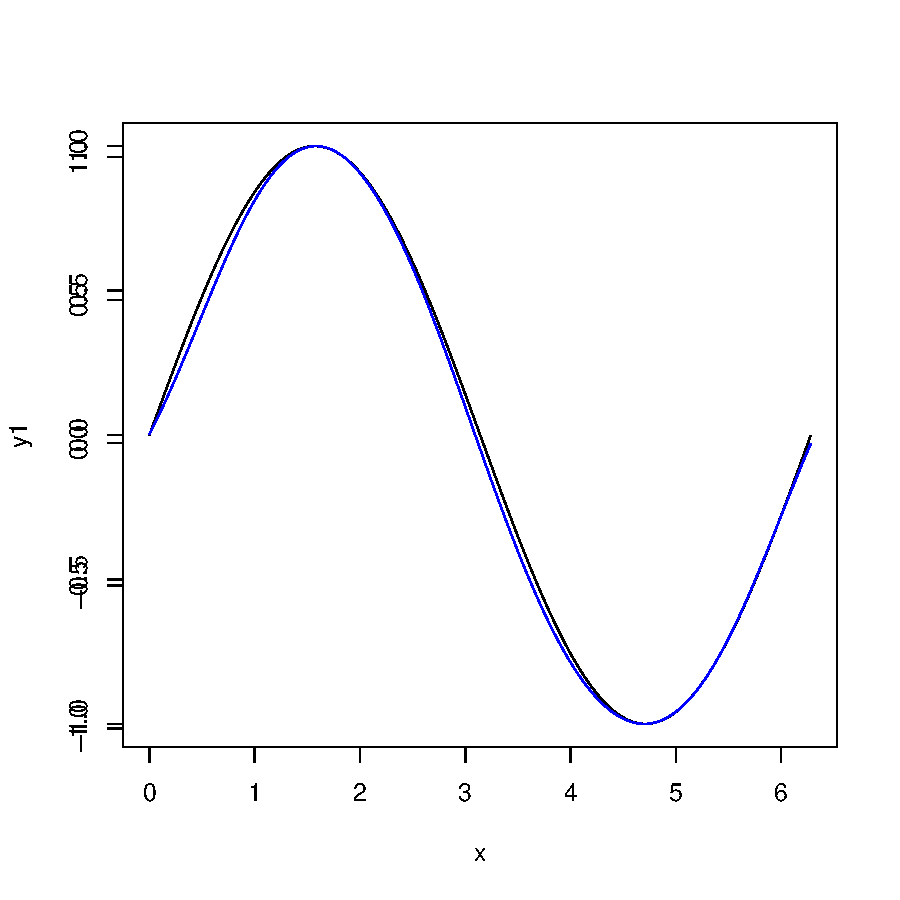
\includegraphics{mlppacotes-004}

A seguir o Método 2 é avaliado, e seu erro apresentado:

\begin{Schunk}
\begin{Sinput}
>   erro2 <- avaliarMetodo2()
>   erro2
\end{Sinput}
\begin{Soutput}
[1] 0.0929663
\end{Soutput}
\end{Schunk}
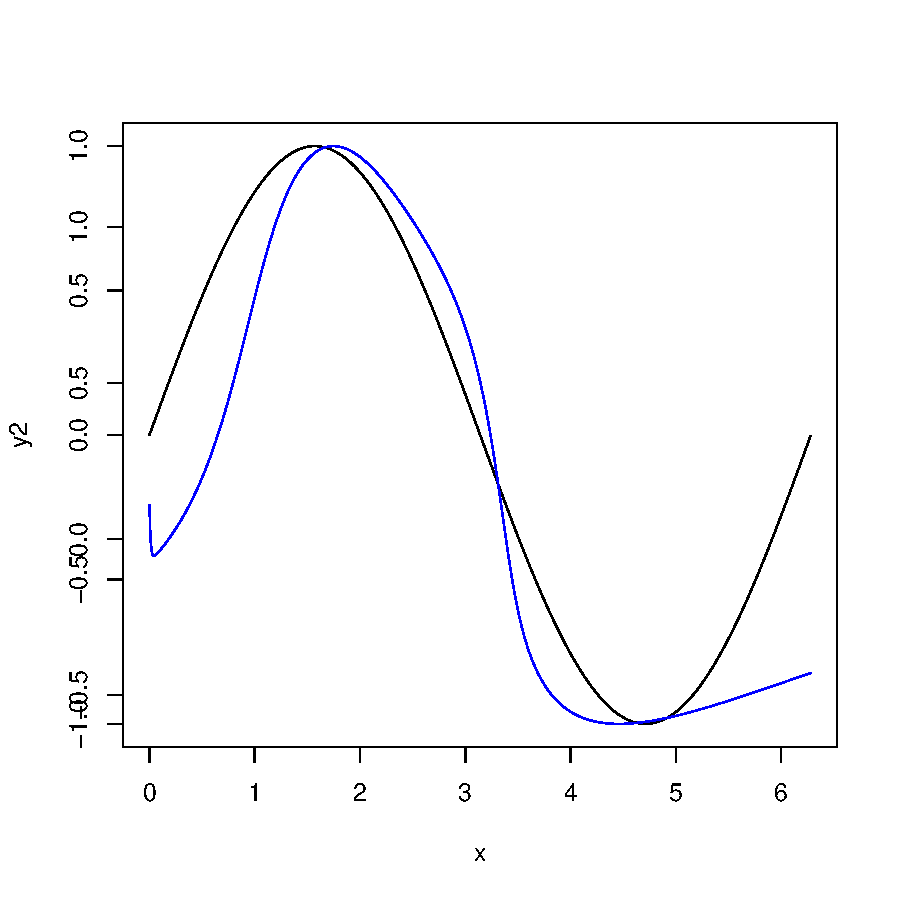
\includegraphics{mlppacotes-005}

A seguir o Método 3 é avaliado, e seu erro apresentado:

\begin{Schunk}
\begin{Sinput}
>   erro3 <- avaliarMetodo3()
\end{Sinput}
\begin{Soutput}
hidden: 3    thresh: 0.01    rep: 1/1    steps:     641	error: 0.64723	time: 0.12 secs
\end{Soutput}
\begin{Sinput}
>   erro3
\end{Sinput}
\begin{Soutput}
[1] 0.03399063728
\end{Soutput}
\end{Schunk}
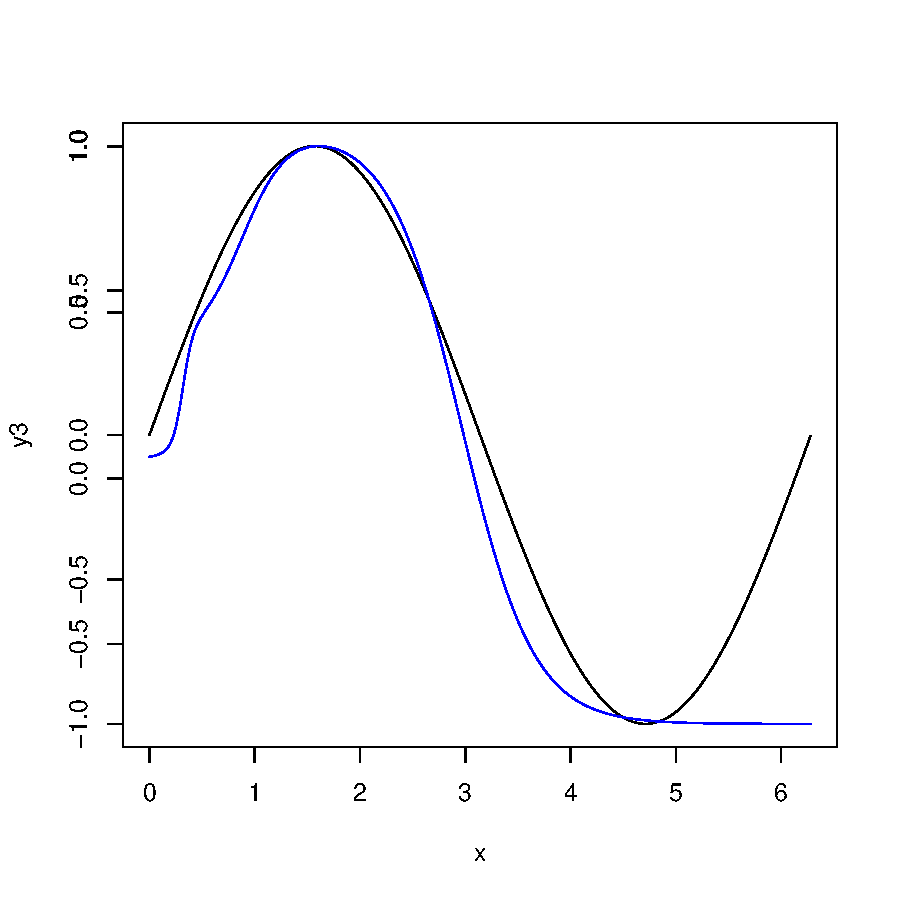
\includegraphics{mlppacotes-006}

\end{document}
